\documentclass{article}

\PassOptionsToPackage{numbers,compress}{natbib}
\newif\ifpublicrelease
\ifdefined\publicrelease
  \publicreleasetrue
\else
  \publicreleasefalse
\fi
\ifpublicrelease
  \usepackage[preprint,sglblindworkshop]{neurips_2026}
\else
  \usepackage[dblblindworkshop]{neurips_2026}
\fi
\workshoptitle{Interpretability as a Science: Toward Rigorous Foundations for Understanding LLMs}

\usepackage[utf8]{inputenc}
\usepackage[T1]{fontenc}
\usepackage{courier}
\usepackage{hyperref}
\hypersetup{
  hidelinks,
  pdftitle={Worse Than Random: J-Space Ablation Is Anti-Selective at Every Measured Qwen3 Scale},
  pdfauthor={Peter Flo},
  pdfsubject={Accepted at the NeurIPS 2026 Workshop on Interpretability as a Science},
  pdfkeywords={mechanistic interpretability, J-space, Jacobian lens, Qwen3, ablation}
}
\usepackage{url}
\usepackage{booktabs}
\usepackage{amsmath}
\usepackage{amsfonts}
\usepackage{graphicx}
\usepackage{microtype}
\usepackage{xcolor}

\graphicspath{{../extension/analysis/}{figures/}}
\newcommand{\jspace}{J-space}
\newcommand{\jlens}{J-lens}
\newcommand{\acc}{\operatorname{Acc}}
\newcommand{\na}{\text{n/a}}

\ifpublicrelease
  \title{Worse Than Random: J-Space Ablation Is Anti-Selective at Every Measured Qwen3 Scale%
    \thanks{Accepted at the NeurIPS 2026 Workshop on Interpretability as a Science.}}
  \author{Peter Flo\\Harvard University\\\href{https://pflo.org}{pflo.org}}
\else
  \title{Worse Than Random: J-Space Ablation Is Anti-Selective at Every Measured Qwen3 Scale}
  \author{Anonymous Authors}
\fi

\begin{document}

\maketitle

\begin{abstract}
The global-workspace interpretation of \jspace{} rests on a selectivity claim: ablating a
model's ``verbalizable'' directions should impair internal reasoning while sparing routine
language. Across a historical 4B pilot and three preregistrations on the open Qwen3 family, we find the opposite
signature at every measured scale. J-ablation damages ordinary-text prediction
\emph{more} than a norm-matched random intervention on 50 of 50, 49 of 50, and 42
of 50 paired WikiText sequences at 1.7B, 14B, and 32B (exact sign tests, $p\le10^{-6}$).
A selectivity index, the ratio of J to matched-random damage, declines
monotonically across the four scales, from 3.38 at 1.7B to 1.16 at 32B, yet never reaches
parity; the 1.7B and 32B endpoints are confirmatory under separate preregistrations. The recorded displacement
norms explain why the control fails: matched perturbation norm at the
injection site does not deliver matched severity. The J-perturbation attenuates
downstream while causing about $2.4\times$ more damage per unit displacement, so
norm-matched random controls are not severity-matched controls. A preregistered
conjunctive validity gate stops at every scale, and two of four stock lenses fail its
lens prerequisite. Because no finished stock 32B lens is available, we fit one from
scratch with the source study's released recipe; the resulting lens, the best-validating in the study,
still yields anti-selectivity. The results do not test
the source study's frontier-scale models: the attenuating index is consistent with
selectivity emerging only beyond 32B, a falsifiable boundary for future instruments.
\end{abstract}

\section{Introduction}

Interventions are central to mechanistic interpretability because they can test whether a
model component plays a causal role rather than merely correlating with behavior
\citep{geiger2021causal}. Yet causality is not the same as construct validity. Removing
any sufficiently large activation component may hurt a task, so an observed drop does not
show that the targeted representation, rather than generic damage, carried the
hypothesized computation. Conversely, a probe can recover information without identifying
a selective mechanism; control tasks are needed to put probe performance in context
\citep{hewitt2019controls}. An intervention-validity claim therefore needs both a positive
effect and discriminant controls.

We study this problem for the Jacobian lens (\jlens{}) and \jspace{} introduced by
\citet{gurnee2026verbalizable}. The \jlens{} maps intermediate residual-stream activations
into final-layer coordinates using an average Jacobian, and its token-indexed directions
define a sparse set of ``verbalizable'' representations. The source study reports that
ablating active \jspace{} directions impairs internal multi-step reasoning while sparing
much routine language processing, one of several functional signatures motivating a
global-workspace interpretation. Selectivity is essential to that interpretation: a
workspace-like channel should not simply be a lossy proxy for the whole residual stream.

This paper reports what happens when that selectivity claim is transferred, without
tuning, to the open Qwen3 family under preregistered conditions. The headline finding is a
sign reversal with a clean scale structure. At every scale where the comparison was
made, removing the ``verbalizable'' directions damages ordinary next-token prediction
\emph{more} than removing an equal-norm random component at the same positions and layers.
The effect is nearly deterministic at 1.7B (worse on all 50 paired sequences), remains
lopsided at 14B (49 of 50), and persists at 32B (42 of 50) under the best-validating lens
in the study. The ratio of J to matched-random damage, an interpretable selectivity
index, falls monotonically with scale (3.38, 2.17, 1.57, 1.16; Figure~\ref{fig:si})
without reaching parity. The 1.7B and 32B endpoints were confirmed under separately
registered hypotheses at $\alpha=.025$; the 4B and 14B values are labeled exploratory.

A second, methodological finding explains why the field's default control missed this.
The random arm is norm-matched per slot, the convention used by the source study itself.
The recorded per-layer displacement norms show that matched norm at the injection site
does not deliver matched severity. The J-perturbation attenuates as it propagates while
the random perturbation persists, yet J-ablation removes about $2.4\times$ more top-1
agreement per unit of delivered displacement (Figure~\ref{fig:disp}). Matching what an
intervention \emph{injects} does not match what it \emph{does}.

Our contributions:
\begin{itemize}
  \item \textbf{An anti-selectivity result with scale structure.} Targeting \jspace{}
    directions damages ordinary text more than matched random damage at every measured
    Qwen3 scale, preregistered-confirmed at both endpoints (1.7B, 32B), with a monotone
    attenuation of the effect toward, but never reaching, parity.
  \item \textbf{A quantified failure of norm-matched controls.} Matched injection norm
    delivered neither matched downstream displacement nor matched damage; we propose the
    relative selectivity index as the severity-robust criterion, and our own data show
    the registered absolute threshold is scale-brittle.
  \item \textbf{A preregistered validity framework, exercised end to end.} A conjunctive
    gate with ordered stopping, run under three frozen preregistrations plus a locked
    historical pilot, with immutable artifacts; no scale passes, so no mechanistic chain-of-thought claim is licensed
    anywhere in the tested family.
  \item \textbf{Instrument findings and artifacts.} Two of four stock lenses fail the
    gate's lens prerequisite and two pass only narrowly, and no finished stock 32B
    lens is available; we fit one from scratch with the source study's released recipe,
    yielding the study's best-validating lens and a reproducible recipe-faithful
    artifact.
\end{itemize}

\paragraph{Related work.}
Causal-abstraction analyses formalize when interventions license mechanistic claims
\citep{geiger2021causal}, and control tasks established that probe accuracy alone does not
identify selective structure \citep{hewitt2019controls}. A growing line of work documents
how intervention evidence can mislead: single directions can spuriously appear to encode
simple concepts \citep{bolukbasi2021illusion}; subspace patching can move behavior through
dormant parallel pathways rather than the hypothesized mechanism
\citep{makelov2023illusion}; and causal localization can fail to predict where editing
works \citep{hase2023localization}. Our study adds the severity dimension: even a
correctly targeted comparison misleads when its control matches perturbation norm rather
than delivered damage. We also exercise a preregistered gate that operationalizes these
concerns as stop rules rather than post-hoc caveats.

\section{Preregistered validity framework}

\subsection{Models, lenses, and the fixed intervention}

We evaluate released Qwen3 checkpoints \citep{qwen3technicalreport} in bfloat16, each
with its matching pretrained \jlens{} from the public fitted-lens repository, a release
distinct from the source study's companion code. All checkpoints, lens files, evaluation code, and datasets are pinned by
immutable revision; Appendix~\ref{app:provenance} lists the identifiers. No model is
trained or fine-tuned.

For layer $\ell$ and residual activation $h_{\ell,t}$, let $J_\ell$ be the average
Jacobian transporting that activation to the final-layer basis. Lens scores are obtained
by applying the model's final normalization and unembedding to $J_\ell h_{\ell,t}$
\citep{gurnee2026verbalizable}. At each token position and intervened layer, following
the source study's ablation protocol \citep{gurnee2026verbalizable}, we select the
$k=10$ tokens ranked highest by this readout, then discard from that set any token among
the parallel clean stream's top ten next-token predictions. If the surviving directions
(at most $k$) are the rows of $V$, our frozen implementation removes their joint
projection in regularized form,
\begin{equation}
  \delta_J = V^\top (VV^\top + \lambda I)^{-1} Vh,
  \qquad h \leftarrow h-\delta_J .
  \label{eq:ablation}
\end{equation}
The intervention runs during prompt processing and generation. A paired clean stream over
the same tokens supplies the exemptions before each intervened forward pass.

The random arm draws $k$ directions per slot from a fixed seeded Gaussian bank
(4{,}096 vectors, sampled with replacement), removes the regularized joint projection
onto them, and rescales the resulting displacement to $\lVert\delta_J\rVert_2$ for the
hypothetical J-ablation at that same slot and state. It therefore controls for local
displacement magnitude without targeting \jlens{} directions, matching the source study's
control convention. In Eq.~\ref{eq:ablation},
$\lambda=10^{-4}\max(\max_i(VV^\top)_{ii},10^{-8})$ is a numerical-stability choice
fixed in our frozen implementation.
The historical 4B band 14--19 is represented as the half-open normalized interval
$[14,20)/36$; multiplying both boundaries by target depth and flooring fixes layers 14--19
at 8B, 15--21 at 14B, 10--14 at 1.7B, and 24--34 at 32B. There is no layer, strength, or
$k$ search at any scale.

\subsection{The gate: ordered measurements and stopping}

Each model proceeds independently through four stages.

\paragraph{1. Lens prerequisite.}
The stock \jlens{} and a logit-lens baseline \citep{nostalgebraist2020logitlens} rank
silent intermediate answers on all 55
order-of-operations and 93 multi-hop items supplied with the source implementation. For at
least one dataset, the \jlens{} must weakly improve mean pass@1 and pass@5, with a strict
improvement on at least one. Otherwise the model is a measurement failure.

\paragraph{2. Clean floor and positive control.}
All 55 order-of-operations prompts receive an eight-token greedy completion. Clean
accuracy must be at least 60\%. We then run J and random arms on the same paired items.
Let $A_C,A_J,A_R$ be their accuracies and $D_J=A_C-A_J$, $D_R=A_C-A_R$. A positive,
J-specific effect requires both two-sided exact McNemar tests \citep{mcnemar1947} to
satisfy $p(C,J)<.05$ and $p(R,J)<.05$, with $A_J<A_R$, and also requires
$D_J\geq2\max(D_R,0)$.

\paragraph{3. Ordinary-text selectivity.}
We deterministically select 50 WikiText-103 training sequences \citep{merity2016wikitext},
truncate each to 128 tokens, and measure teacher-forced top-1 agreement with the clean
model over the resulting 6,400 positions. J-ablation must preserve strictly more than
80\%. The random arm is retained as the matched-severity comparator.

\paragraph{4. Coherence.}
Only a model clearing all earlier conditions generates non-thinking chain-of-thought on 30
fixed GSM8K training problems \citep{cobbe2021gsm8k}. Fewer than 10\% may hit the
640-token cap or exceed 0.5 maximum four-gram repetition fraction. Passing the study means
satisfying \emph{every} condition. For reported effect sizes we use 10,000 paired item or
sequence bootstrap draws with seed 20260825; early-stopped quantities remain missing
rather than being imputed.

\subsection{One historical pilot, three registrations}

The evidence accumulated under one hash-pinned historical pilot and three frozen
registrations. Each registration was committed with hashed configuration before its runs
and states explicitly that it was written knowing the earlier outcomes (Appendix~\ref{app:v3}).
\textbf{v1 (historical).} A 4B pilot with a calibration ladder; its light-band rung
(layers 14--19, $k=10$) supplies the transferred intervention and is treated as
descriptive context only. \textbf{v2.} The frozen transfer to 8B (secondary) and 14B
(primary) with the complete gate and ordered stops. \textbf{v3.} The two reserved scales,
1.7B and 32B, with one registered procedural change: every non-coherence stage is measured
even when a prerequisite fails, so the selectivity comparison cannot be censored the way
the 8B stop censored it. Anti-selectivity is the confirmatory primary endpoint (exact sign
test on the 50 paired per-sequence differences and a bootstrap selectivity-index interval
excluding one, $\alpha=.025$ per model). \textbf{v4.} The 32B arm, blocked in v3 because
no finished stock 32B lens is available, completed by fitting
the lens from scratch with the recipe released in the source study's companion
implementation, at the pinned revision (Appendix~\ref{app:v3}); endpoints identical to v3.

\section{Results}

\subsection{The gate stops at every scale; the instruments are the first casualty}

Table~\ref{tab:results} reports the complete registered outcomes and
Table~\ref{tab:checks} the component checks. No scale passes the conjunctive gate. The
stock lenses fail the lens prerequisite at 1.7B and 8B (and the 8B run, under v2 rules,
therefore has no downstream data); the 4B and 14B stock lenses pass narrowly. At 32B the
from-scratch recipe fit passes decisively, with pass@1 of .109 against the logit lens's
.009 on order-of-operations, the widest margin in the study (Table~\ref{tab:lens});
instrument quality therefore cannot explain the 32B outcomes. The upstream 32B artifact itself is an
instrument finding: the fitted-lens repository's sole 32B file contains fitting
state for 80 of a nominal 1,000 prompts rather than a finished lens. That repository's head
equals the pinned revision, so before this study no finished stock 32B lens was available
(Appendix~\ref{app:v3}).

\begin{table}[t]
  \caption{Complete registered outcomes. ``Spec.'' is $A_R-A_J$ with a paired bootstrap
  95\% interval; $p_{CJ}/p_{RJ}$ are two-sided exact McNemar values. The 4B row is
  historical context. Dashes at 8B are required by the v2 ordered stop; the v3/v4 rows
  measure downstream stages regardless of lens outcome. The 32B lens is the
  from-scratch recipe fit.}
  \label{tab:results}
  \centering
  \small
  \begin{tabular}{lcccccc}
    \toprule
    Model & Lens & $A_C/A_J/A_R$ & Spec. [95\% CI] & $p_{CJ}/p_{RJ}$ & Wiki J/R & Gate \\
    \midrule
    1.7B (v3)  & fail & .600/.564/.545 & $-.018$ [$-.055$,.000] & .69/1.0 & .617/.887 & stop \\
    4B (hist.) & pass & .745/.582/.745 & .164 [.073,.273] & .012/.004 & .661/.844 & stop \\
    8B (v2)  & fail & \na & \na & \na & \na & stop \\
    14B (v2) & pass & .836/.818/.836 & .018 [$-.036$,.073] & 1.0/1.0 & .766/.851 & stop \\
    32B (v4) & pass & .836/.764/.836 & .073 [$-.018$,.164] & .22/.29 & .664/.710 & stop \\
    \bottomrule
  \end{tabular}
\end{table}

On the causal side, the positive-control evidence never certifies a J-specific effect
after the pilot. At 14B the drop is 1.8 points with three discordant items ($p=1.0$). At
32B the drop is 7.3 points against a random drop of exactly zero, the largest and most
direction-consistent estimate since the 4B pilot. With $p_{CJ}=.22$ at $n=55$ it
nevertheless remains uncertifiable; Section~\ref{sec:limits} quantifies why this design cannot certify
drops below eleven points. On the selectivity side, the registered absolute threshold
fails everywhere, and at 32B it fails \emph{for both arms}: even random ablation preserves
only .710 of clean predictions there. The absolute bar conflates base-model fragility with
intervention selectivity, which motivates the relative criterion that follows.

\subsection{Anti-selectivity: the targeted directions carry ordinary-language load}
\label{sec:anti}

\begin{figure}[t]
  \centering
  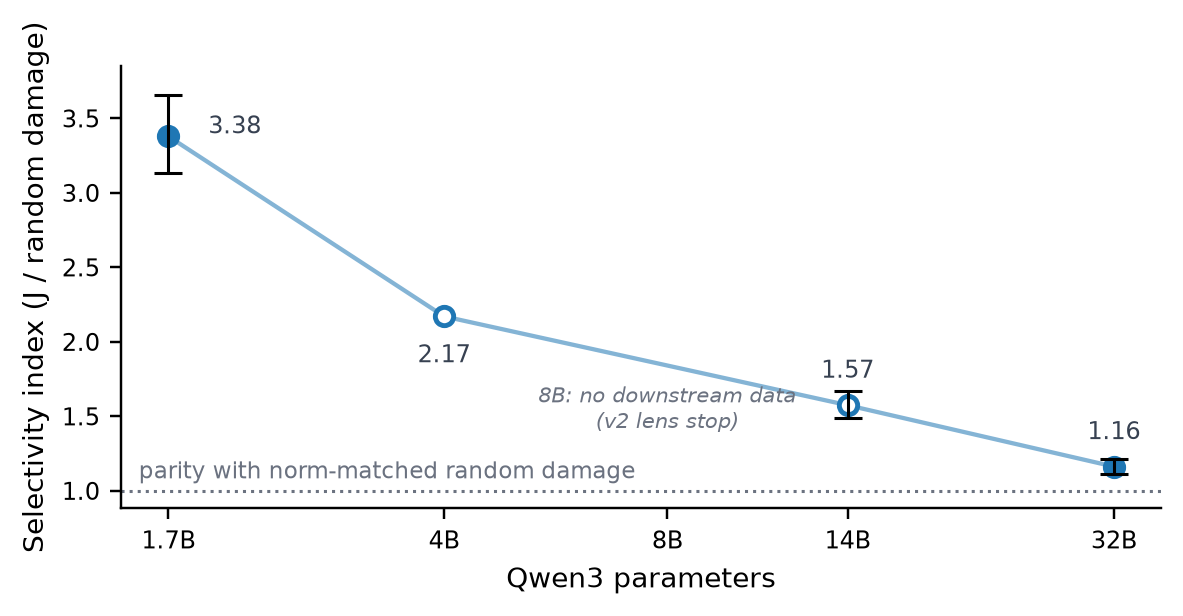
\includegraphics[width=0.86\linewidth]{si_scale.png}
  \caption{The selectivity index (mean J-arm disagreement over mean matched-random
  disagreement on paired WikiText) declines monotonically with scale but never reaches
  parity. Filled markers are confirmatory under a registration written before the run
  (1.7B, 32B; $\alpha=.025$); open markers are exploratory (4B point estimate, 14B).
  Error bars are paired sequence-bootstrap 95\% intervals; the 32B interval is narrower
  than its marker, so only its caps are visible.}
  \label{fig:si}
\end{figure}

\begin{figure}[t]
  \centering
  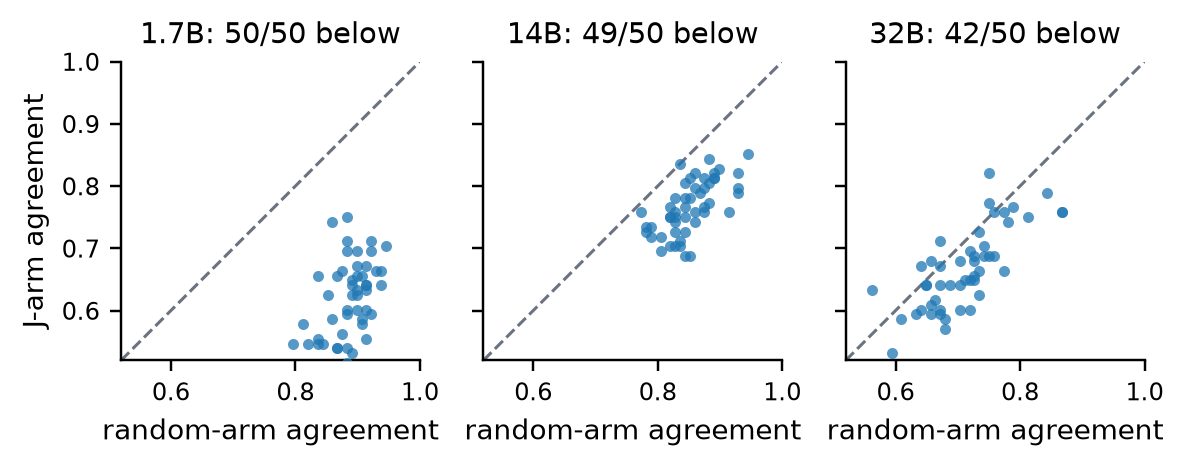
\includegraphics[width=0.92\linewidth]{paired_scatter.png}
  \caption{Per-sequence paired evidence. Each point is one WikiText sequence; below the
  diagonal, J-ablation agrees with the clean model less than the norm-matched random arm
  on the same sequence. Exact sign tests: $p=1.8\times10^{-15}$ (1.7B),
  $3.6\times10^{-15}$ (14B), $1.0\times10^{-7}$ (32B).}
  \label{fig:scatter}
\end{figure}

The workspace interpretation predicts the J arm should damage ordinary text \emph{less}
than matched random damage. The data show the opposite, at every scale with paired data
(Figure~\ref{fig:scatter}): J-ablation agrees less with the clean model on 50 of 50 paired
sequences at 1.7B (no tie broken in its favor), 49 of 50 at 14B (one tie), and 42 of 50 at
32B. As a severity-robust summary we use the selectivity index, the ratio of mean top-1
disagreement rates, $\mathrm{SI}=(1-a_J)/(1-a_R)$; values above one mean the targeted
intervention damages ordinary prediction more than matched damage.
Table~\ref{tab:si} and Figure~\ref{fig:si} give the complete picture: $\mathrm{SI}=3.38$
[3.13, 3.65] at 1.7B, 2.17 at 4B, 1.57 [1.49, 1.67] at 14B, and 1.16 [1.11, 1.21] at 32B.
The 1.7B and 32B values confirm the registered anti-selectivity hypothesis at
$\alpha=.025$ each (sign tests above; interval excluding one); the mean paired deficits
are $-27.0$ points [$-28.6,-25.3$] and $-4.7$ points [$-6.0,-3.3$].

\begin{table}[t]
  \caption{Selectivity index across all frozen interventions. The 1.7B and 32B rows are
  confirmatory under the v3/v4 registrations; the others are exploratory. The 32B row
  uses the from-scratch recipe fit.}
  \label{tab:si}
  \centering
  \small
  \begin{tabular}{llccc}
    \toprule
    Model & Band & $k$ & Wiki J/R & SI [95\% CI] \\
    \midrule
    1.7B (v3) & 10--14 & 10 & .617/.887 & 3.38 [3.13, 3.65] \\
    4B & 14--24 & 10 & .617/.792 & 1.84 \\
    4B & 14--31 & 10 & .577/.728 & 1.55 \\
    4B & 14--24 & 5  & .610/.817 & 2.13 \\
    4B & 14--19 & 10 & .661/.844 & 2.17 \\
    14B & 15--21 & 10 & .766/.851 & 1.57 [1.49, 1.67] \\
    32B (v4) & 24--34 & 10 & .664/.710 & 1.16 [1.11, 1.21] \\
    \bottomrule
  \end{tabular}
\end{table}

Two properties of this pattern deserve emphasis. First, it is not a threshold artifact:
the paired, relative comparison is decisive at every scale even where the registered
absolute bar is uninformative. Second, the monotone attenuation
(3.38 $\rightarrow$ 2.17 $\rightarrow$ 1.57 $\rightarrow$ 1.16, under the matched
transfer band and $k$) is a descriptive trend, not a registered contrast: it is
consistent with ordinary-language load gradually disentangling from the
\jspace{} directions as capacity grows. Equally, it bounds where workspace-style
selectivity could first appear: strictly above 32B in this family, if anywhere. Scale is
confounded with architecture, lens estimation, and how well the normalized-depth band
transfers, so we treat the trend as a falsifiable boundary rather than a mechanism claim.

\subsection{Matched norm is not matched damage}
\label{sec:severity}

\begin{figure}[t]
  \centering
  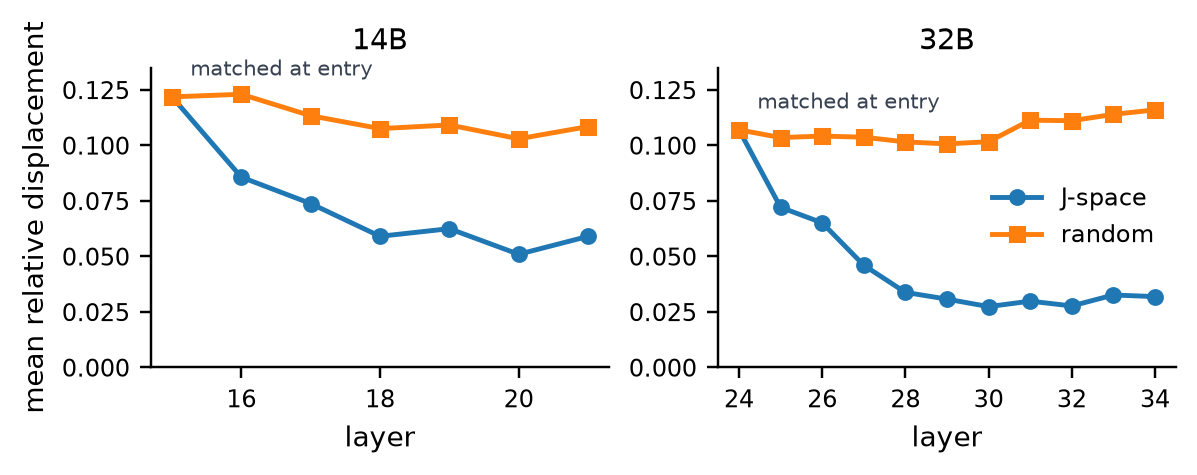
\includegraphics[width=0.9\linewidth]{displacement.png}
  \caption{Mean per-layer relative displacement of the two WikiText arms (frozen values).
  Both arms are norm-matched at the band's entry layer, but the J-perturbation attenuates
  as it propagates while the random perturbation persists, at both 14B and the
  from-scratch-fit 32B. The arm with the \emph{smaller} delivered displacement causes the
  \emph{larger} damage.}
  \label{fig:disp}
\end{figure}

Why does the field's standard control miss this? The recorded per-layer displacement
norms give a mechanical answer (Figure~\ref{fig:disp}). At 14B the two arms enter the band
with displacement matched to within one part in $10^{8}$, but the J displacement attenuates
through it (last-to-first-layer ratio .48 versus .89 for random). The result is a smaller
cumulative displacement (.51 versus .79) yet larger damage: about $2.4\times$ more lost
top-1 agreement per unit of displacement (Appendix Table~\ref{tab:displacement}). The
same dissociation appears at 32B, where the J displacement decays to roughly a quarter of
the persisting random displacement while still causing more damage. Norm-matching at the
injection site therefore delivers neither matched downstream displacement nor matched
damage, and displacement alone does not account for the difference. Any study that
certifies selectivity with a norm-matched random control inherits this gap; the paired
relative criterion of Section~\ref{sec:anti} does not.

\subsection{Item anatomy and the limits of the causal design}
\label{sec:limits}

Item-level hit vectors refine the historical comparison. At 4B the same nine control
items flip from correct to incorrect under every calibration rung (pairwise Jaccard
.82--1.0 against a chance expectation near .14). The random arms also concentrate on this
stable set (10 of their 14 down-flips), so the core marks items generally fragile
under band perturbation; what distinguishes J-ablation is flipping the complete set at
every dose. The two 14B down-flips avoid the core entirely, and the 1.7B and 32B arms each place
only one of their four and five down-flips in it (exact hypergeometric tails $p=.42$ and
$p=.58$ over each model's clean-correct items). There is therefore no positive evidence
that the later point estimates are the 4B effect attenuated, though the design cannot
rule that reading out (Appendix~\ref{app:explore}).

The causal arm's resolution is bounded by design: with $n=55$ paired items, exact
two-sided McNemar cannot reach $p<.05$ with fewer than six discordant items all in one
direction, so no observed drop below 10.9 points is certifiable. The same design did
detect the historical 16.4-point effect, and the 14B interval excludes a J-specific
effect of that size; the suggestive 7.3-point 32B estimate sits squarely in the
uncertifiable zone. Limited power therefore qualifies conclusions about small effects,
not about the effect that motivated the transfer.

\section{What the evidence licenses}

\paragraph{A stopped experiment can be a result.}
The negative conclusion depends on preserving the order of inference. Had we ignored the
lens failures, selected different layer bands after seeing results, or proceeded from
uncertified point estimates to downstream outcomes, the same data could support a much
more fluent but weaker story. The preregistered gate instead distinguishes measurement
failure (1.7B, 8B lenses), minimal instrument adequacy (4B, 14B), decisive instrument
adequacy (the 32B refit), and intervention invalidity (everywhere). The unrun coherence
and chain-of-thought quantities are outside the evidence, not null effects.

\paragraph{This is not a causal claim about parameter count, and not a test of the
source models.}
Model scale varies together with architecture, representation geometry, lens estimation
quality, and how well a normalized-depth band targets the relevant computation. The
attenuating selectivity index is consistent with workspace-style selectivity emerging
only at scales beyond 32B, where the source study's frontier models live. Nothing here
tests those models, and the source claims remain open and newly testable: the index
gives any larger open model with a fitted lens a concrete parity criterion. Within the
tested family, the conclusion is pipeline-conditional but uniform: increasing Qwen3 scale
to 32B does not deliver the selectivity signature, and the ``verbalizable'' directions
carry measurable ordinary-language load everywhere.

\paragraph{Matched damage and preservation answer different questions.}
The random arm asks whether a positive-control effect is special to the proposed
directions; WikiText asks whether those directions are restricted to the hypothesized
class of computation. At every measurable scale the random arm preserves more
ordinary-text predictions than J-ablation, while no scale certifies a J-specific control
effect. Neither substitutes for the other, and the conjunctive logic is portable to other
activation interventions even when the particular thresholds are not; our own data argue
the selectivity criterion should be the relative index rather than an absolute bar.

\section{Limitations and broader impact}

The study covers one model family, four evaluated transfer scales, one transferred band,
one $k$, and one intervention style. The 32B arm uses a lens we fit ourselves, albeit
with the released recipe to the released convergence standard, and its outcomes are
labeled accordingly. The 55-item positive control yields coarse effect resolution
(Section~\ref{sec:limits}). The 80\% text threshold and lens-ranking rule are operational
validity criteria, not universal definitions of a mechanism, and the 32B data show the
absolute threshold conflates fragility with selectivity. The exploratory analyses
(Sections~\ref{sec:severity} and~\ref{sec:limits} in part) were computed after registered
outcomes were known and are labeled throughout; the selectivity index originated that way
before becoming the registered v3/v4 endpoint. The 4B row is historical rather than
preregistered. A separately registered study could test alternative lenses, bands, or
families, but selecting them because these outcomes are inconvenient would be exploratory
evidence.

The work introduces no model capability and uses public checkpoints and datasets. Its
main positive impact is methodological: severity-matched controls and stopping rules
reduce the risk that generic intervention damage is reported as mechanistic
understanding, and the from-scratch recipe fit adds a validated 32B lens to the public
instrument ecosystem. A possible negative impact is overgeneralizing one failed
operationalization into a claim that the underlying mechanism does not exist anywhere; we
mitigate this by confining every conclusion to the tested pipeline and family and by
stating explicitly what remains untested.

\section{Conclusion}

Ablation-induced behavior change is not enough, and at these scales the change itself
tells the opposite story. Under a frozen transfer across the Qwen3 family, the
``verbalizable'' directions damage ordinary language more than norm-matched random damage
at every measured scale, confirmatory at both registered endpoints, while the effect
attenuates monotonically toward, but never reaches, parity. The gate stops everywhere, so
no mechanistic chain-of-thought claim is licensed in this family, and the norm-matched
control convention is shown to under-match severity by a factor of about $2.4$. The
question the source study raised now has a sharp, portable form: if workspace selectivity
is real, its parity crossing lies above 32B, waiting for the next instrument.

\bibliographystyle{plainnat}
\bibliography{references}

\appendix

\section{Registered gate and component outcomes}
\label{app:gate}

Table~\ref{tab:checks} shows every component of the conjunction. A blank entry means the
ordered procedure stopped before that component (v2) or that the stage is unreachable by
rule (coherence, whenever any earlier condition fails). The historical 4B row is
evaluated against the version-2 gate only for descriptive comparability. ``J effect''
denotes $D_J>0$ with $p_{CJ}<.05$; ``J$<$R'' also includes $p_{RJ}<.05$. ``Ratio''
denotes $D_J\geq2\max(D_R,0)$.

\begin{table}[ht]
  \caption{Component checks for the complete gate. The 32B row uses the from-scratch recipe
  fit.}
  \label{tab:checks}
  \centering
  \small
  \begin{tabular}{lccccccc}
    \toprule
    Model & Lens & Clean & J effect & J$<$R & Ratio & Wiki & Coherence \\
    \midrule
    1.7B (v3) & fail & pass & fail & fail & fail & fail & \na \\
    4B (hist.) & pass & pass & pass & pass & pass & fail & pass \\
    8B (v2) & fail & \na & \na & \na & \na & \na & \na \\
    14B (v2) & pass & pass & fail & fail & pass & fail & \na \\
    32B (v4) & pass & pass & fail & fail & pass & fail & \na \\
    \bottomrule
  \end{tabular}
\end{table}

The registered v2 visualization of the 8B/14B outcomes is reproduced in
Figure~\ref{fig:v2gate} for provenance; its analysis directory is locked and unchanged.

\begin{figure}[ht]
  \centering
  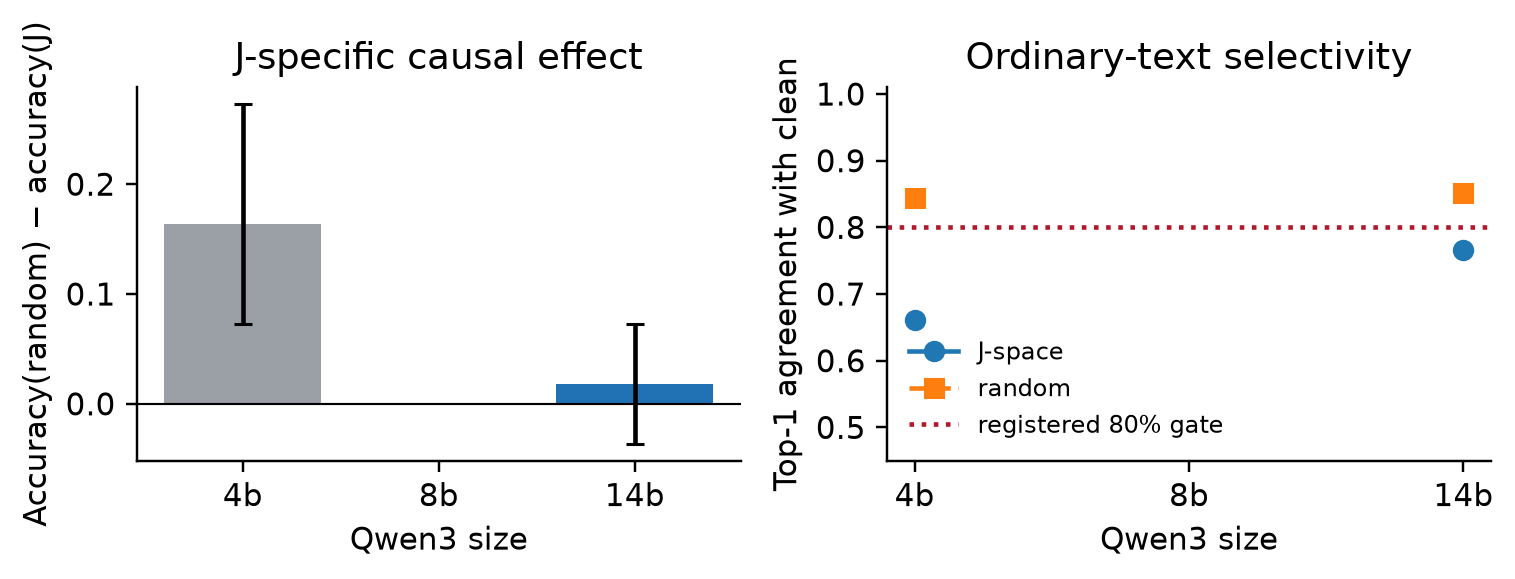
\includegraphics[width=\linewidth]{scale_gate.png}
  \caption{The locked v2 analysis figure (4B historical, 8B, 14B): J-specific
  positive-control effect (left) and ordinary-text selectivity against the registered
  80\% bar (right). Error bars are paired bootstrap 95\% intervals.}
  \label{fig:v2gate}
\end{figure}

\section{Lens-validation detail}
\label{app:lens}

The gate uses pass@1 and pass@5 only; pass@10 is reported for completeness. It passes when
the \jlens{} weakly exceeds the logit lens at both registered ranks and strictly exceeds it
at one, on either dataset. The 32B rows use the from-scratch recipe-fit lens.

\begin{table}[ht]
  \caption{Mean fraction of target intermediates recovered within rank $k$.}
  \label{tab:lens}
  \centering
  \small
  \begin{tabular}{llcccccc}
    \toprule
    & & \multicolumn{3}{c}{\jlens{}} & \multicolumn{3}{c}{Logit lens} \\
    \cmidrule(lr){3-5}\cmidrule(lr){6-8}
    Model & Dataset ($n$) & @1 & @5 & @10 & @1 & @5 & @10 \\
    \midrule
    1.7B & order-ops (55) & .109 & .191 & .364 & .155 & .245 & .318 \\
         & multi-hop (93) & .140 & .301 & .398 & .161 & .296 & .387 \\
    8B & order-ops (55) & .055 & .291 & .418 & .182 & .355 & .473 \\
       & multi-hop (93) & .156 & .387 & .462 & .215 & .409 & .471 \\
    14B & order-ops (55) & .073 & .255 & .391 & .036 & .209 & .309 \\
        & multi-hop (93) & .140 & .349 & .557 & .145 & .366 & .471 \\
    32B (refit) & order-ops (55) & .109 & .318 & .418 & .009 & .209 & .282 \\
        & multi-hop (93) & .220 & .482 & .622 & .154 & .498 & .541 \\
    \bottomrule
  \end{tabular}
\end{table}

\section{Exploratory-reanalysis detail}
\label{app:explore}

The exploratory quantities in Sections~\ref{sec:anti}--\ref{sec:limits} are recomputed by
the deterministic supplement script \texttt{jspace.frozen\_explore} (bootstrap seed
20260825, 10{,}000 draws) from three immutable inputs: the registered 14B result artifact
and the two historical 4B calibration files. The script records the inputs' SHA-256
digests in its output and asserts agreement with the registered McNemar values before
reporting. Because the registered outcomes were known when these analyses were chosen,
they are exploratory under our own standard; the selectivity-index estimator defined here
was subsequently registered verbatim as the v3/v4 primary endpoint. The analyses reported
here and in the main text are the complete set of post-hoc analyses performed on the
frozen artifacts; none was run and withheld.

The selectivity index is the ratio of mean top-1 disagreement rates, J-ablation over
norm-matched random. Intervals are percentile bootstrap over the 50 paired sequences (the
random-arm disagreement is bounded away from zero, so the ratio is well behaved under
resampling); per-sequence agreements were not retained in the 4B artifacts, so the 4B
rungs carry point estimates only.

\begin{table}[ht]
  \caption{Mean per-layer relative displacement of the 14B WikiText arms (frozen values).
  ``Dose'' is the sum over band layers, a coarse severity proxy; ``damage'' is one minus
  top-1 agreement with the clean model. The corresponding 32B profile appears in
  Figure~\ref{fig:disp}.}
  \label{tab:displacement}
  \centering
  \small
  \begin{tabular}{lcccccccccc}
    \toprule
    Arm & 15 & 16 & 17 & 18 & 19 & 20 & 21 & Dose & Damage & Damage/dose \\
    \midrule
    J      & .122 & .086 & .074 & .059 & .062 & .051 & .059 & .513 & .234 & .456 \\
    Random & .122 & .123 & .113 & .108 & .109 & .103 & .108 & .786 & .149 & .189 \\
    \bottomrule
  \end{tabular}
\end{table}

Down-flips are items the clean model answers correctly and an intervened arm answers
incorrectly, indexed by dataset file order. The 4B core comprises the nine items the J arm
flips under all four calibration rungs; exact hypergeometric tail probabilities for the
observed pairwise overlaps, taken over the 41 clean-correct items, are at most
$3\times10^{-7}$. The equal-norm random arms flip 5, 5, 3, and 1 items across the same
rungs, and 10 of those 14 down-flips are core items where the exchangeable null expects
about three, so the core also marks items generally fragile under band perturbation. The
hypergeometric null treats items as exchangeable; these statistics therefore establish a
stable, rung-independent flip set that J-ablation saturates at every dose, not targeting
per se. The later J-arm down-flips avoid or barely touch the core: 0 of 2 at 14B, 1 of 4 at
1.7B, and 1 of 5 at 32B (with 4 and 7 of the nine core items clean-correct at 1.7B and
32B, the exact tails over their 33 and 46 clean-correct items are $p=.42$ and $p=.58$;
the 14B overlap of zero admits no tail below one): weak evidence either way,
offering no positive support for reading the later point estimates as the 4B effect
attenuated, though it cannot rule that reading out. Cross-model comparison assumes all
studies stage the pinned evaluation file in file order; within-4B comparisons need no
such assumption.

Design limits of the registered test: with $n=55$ paired items, exact two-sided McNemar
cannot reach $p<.05$ with fewer than six discordant items all in one direction (a
10.9-point observed drop); five one-way discordant items give $p=.0625$, and eight versus
one gives $p=.039$. The design was therefore sensitive to the historical 16.4-point
effect (ten versus one discordant, $p=.012$) but cannot certify drops below roughly
eleven points, including the 7.3-point 32B estimate (five versus one discordant,
observed $p_{CJ}=.22$; even a five-versus-zero split would give only $p=.0625$).

\section{The version-3 and version-4 registrations and outcomes}
\label{app:v3}

\paragraph{Version 3.}
The third registration was frozen and committed before any 1.7B or 32B staging or
inference; its SHA-256 digests are \texttt{24a1d8d7\ldots{}c993} (preregistration) and
\texttt{3e3b553e\ldots{}28c8} (configuration). It states explicitly that it was written
with the v2 outcomes and the exploratory reanalysis known, covers exactly the two models
the v2 preregistration reserved for separate recording, and reuses the v2 thresholds,
datasets (the staged-data digest reproduces), $k$, exemption, seeds, and band rule. Its
one registered procedural change measures every non-coherence stage even when an earlier
prerequisite fails; the conjunctive gate verdict is unchanged. Registered endpoints: the
anti-selectivity prediction as confirmatory primary (exact sign test on the 50 paired
per-sequence differences and a bootstrap selectivity-index interval excluding one, at
$\alpha=.025$ per model), the complete gate as secondary, and a conditional flip-core
overlap test. Descriptive intervals in the 1.7B and 32B rows follow the v2 reporting
convention; they were added to the summary script after the 1.7B data existed and feed no
registered endpoint. A second post-data correction to the same script fixed the H4
hypergeometric population to match the registered wording (the marked class is the core
items clean-correct at that model), moving the 1.7B tail from .74 to .42 without changing
the no-signal conclusion; both changes are deviation-logged, and the registered H1
outputs are byte-identical to the pre-data script.

At 1.7B the stock lens fails on both datasets (Table~\ref{tab:lens}), clean control
accuracy sits exactly at the .60 floor, J-ablation removes 3.6 points against the random
arm's 5.5 ($p_{CJ}=.69$, $p_{RJ}=1.0$), and WikiText agreement is .617 under J against
.887 under random; the gate stops before coherence. The primary endpoint confirms
decisively (Section~\ref{sec:anti}). The 32B arm could not run under v3: the pinned lens
file contains \texttt{fit()} state rather than a finished lens (raw
\texttt{jacobian\_sum} over 63 source layers, \texttt{n\_done}~$=80$ prompts), its convergence log ends
at prompt 80 with delta near $.03$ where the released recipe stops at $.002$, and the
repository head is identical to the pinned revision, so no finished stock 32B lens exists
in that repository.

\paragraph{Version 4.}
The fourth registration (digests \texttt{4c771fc1\ldots{}e054} and
\texttt{9997bb6f\ldots{}0825}) authorizes exactly one act of instrument construction:
fitting the 32B lens from scratch with the recipe released in the source study's
companion code: wikitext-103 train prompts in dataset order (first 1{,}000 rows with at least 600
stripped characters, truncated to 2{,}000 characters; eligible ranks 0--999, disjoint by
construction from the evaluation slice, which skips the first 2{,}000 eligible rows),
\texttt{max\_seq\_len} 128, bfloat16, with the released early stop reimplemented as a
registered block rule (stop at the first multiple of 10 prompts at or beyond 100 where
the running mean changed by less than 0.02, maximum over layers, across the preceding 10
prompts). The fit converged by that rule at 760 prompts; the finished lens is saved in
the stock format with SHA-256 \texttt{3efa365d\ldots{}3c0e}, recorded together with its
convergence trace in a committed manifest, and the gate result records the override file
and digest. Two execution deviations are logged: the Jacobian chunk width ran at 16
rather than the released 128 (the released fit used a 179~GB accelerator; the width only
partitions the identical computation), and the fit consumed 32.3 GPU-hours against its
registered 30-hour cap because the driver's wall guard was set to the job limit rather
than the cap; the error is recorded in the deviation log and was not an outcome-driven
choice. Endpoints are identical to v3; the 32B outcomes are reported in
Sections~\ref{sec:anti}--\ref{sec:limits} and are never merged into stock-lens rows
without the refit label.

Beyond the fit itself, version-3 execution used 3.47 GPU-minutes (a 13-second smoke, a
7-second pre-data provenance stop that was deviation-logged and resubmitted unchanged,
the registered 1.7B gate at 2\,min\,31\,s on one L40S at 3.61\,GB peak, and the
37-second 32B smoke that surfaced the 32B instrument finding), and version-4
gate-stage execution used 8.5 GPU-minutes (a 55-second smoke and the 7\,min\,34\,s
registered gate at 66.4\,GB peak on one H200). Three pre-fit infrastructure failures (4,
40, and 23 seconds) read no registered data and are deviation-logged.

\section{Provenance, execution, and reproducibility}
\label{app:provenance}

The v2 preregistration, machine-readable configuration, runner, and locked analysis were
committed before registered inference; the preregistration and configuration have SHA-256
digests \texttt{354ce44f\ldots{}548a} and \texttt{18581126\ldots{}9b5f}. Registered v2
inference used code commit \texttt{b8f8b624\ldots{}3938}, staged-data digest
\texttt{a7f2abfe\ldots{}81c6}, and the following immutable public revisions:
\begin{itemize}
  \item Qwen3-1.7B: \texttt{70d244cc\ldots{}ad5e}; Qwen3-8B: \texttt{b968826d\ldots{}1218};
  \item Qwen3-14B: \texttt{40c06982\ldots{}3e18}; Qwen3-32B: \texttt{9216db57\ldots{}6137};
  \item fitted \jlens{} repository: \texttt{0731326e\ldots{}b3a6}; and
  \item the source study's companion code and synthetic evaluation data:
    \texttt{581d3986\ldots{}ba8e}.
\end{itemize}

Both v2 registered jobs requested and received one NVIDIA L40S, four CPU cores, and 96 GB
host memory, using PyTorch 2.13.0, CUDA 13.0, and bfloat16 weights. Each queued for 37
seconds. The 8B run lasted 3:01 and peaked at 16.47 GB allocated CUDA memory; the 14B run
lasted 6:21 and peaked at 30.13 GB. v2 registered allocation was 9 min 22 s, well below
the preregistered 12 GPU-hour cap; v2 readiness added 1 min 16 s, with the pre- and
post-freeze smoke failures and the offline lens-loading fix recorded in the deviation
log. The v3 and v4 stages appear in Appendix~\ref{app:v3}; the full project total across
the pilot follow-ups and three registrations, including the one-time 32B lens fit, is
32.7 GPU-hours, of which registered gate inference is 19.4 GPU-minutes. Scheduler logs for every registered job
were read in full; none contained an exception, warning, out-of-memory event, or
numerical-error marker.

A public reproducibility release contains the v2, v3, and v4 preregistrations and configurations,
source, dependency lock, item-level paired hit vectors, per-sequence WikiText agreements,
displacement summaries, result JSONs, the refit-lens manifest and recipe, and commands
for staging public data, running the gates, refitting the lens, and reproducing every
table, figure, and registered endpoint evaluation. Host and scheduler identifiers are
omitted from public artifacts; scientific fields and early-stopped values are retained.

\section{Assets and licenses}
\label{app:assets}

Qwen3-1.7B, 8B, 14B, and 32B are released under Apache-2.0. The source study's companion Jacobian-lens
code and synthetic evaluation prompts are Apache-2.0; the fitted lens repository is MIT.
WikiText is listed under CC BY-SA 3.0 and GFDL, and GSM8K under MIT. The supplement
redistributes only our code and derived result artifacts; model weights, prompts, and
corpus text are staged from their original repositories. The from-scratch 32B recipe fit is
reproducible from the committed driver, staged-prompt digest, and manifest; its binary is
not redistributed because of its size.

\section{Use of language-model assistance}
\label{app:llm}

Language-model coding assistants supported software implementation, tests, documentation,
and prose editing. They were not an experimental condition, did not score any outcome,
and could not alter frozen configurations during registered jobs. Scientific failures
were retained rather than tuned or rerun. The human authors remain responsible for
reviewing the code, raw artifacts, statistical outputs, prose, figures, and every cited
source before submission.

\end{document}
